\documentclass{beamer}
\usetheme{ConnectivityLab}
\usepackage{times}
\usepackage{graphicx}
\usepackage{verbatim}
\usepackage{outlines}
\usepackage{fancyhdr}
\usepackage{subfigure}
\usepackage{cancel}
\usepackage{bibentry}
\usepackage{varwidth}
\usepackage{etoolbox}
\usepackage{epstopdf}

%%%%%%%%%%%%%%%%%%%%%%%%%%%%%%%%%%%%%%%%%%%%%%%%%%%%%%
%%%%%%%%%%%%%%%%%%%%%%%%%%%%%%%%%%%%%%%%%%%%%%%%%%%%%%

\title {
    Efficient LTE Access with Collision Resolution for Massive M2M Communications \cite{ELACR}
}
\author {
    Yin-Hong, Hsu
}
\date {
    10 11, 2016
}

%%%%%%%%%%%%%%%%%%%%%%%%%%%%%%%%%%%%%%%%%%%%%%%%%%%%%%
%%%%%%%%%%%%%%%%%%%%%%%%%%%%%%%%%%%%%%%%%%%%%%%%%%%%%%

\begin{document}
\begin{frame}
    \titlepage
\end{frame}

%%%%%%%%%%%%%%%%%%%%%%%%%%%%%%%%%%%%%%%%%%%%%%%%%%%%%%
%%%%%%%%%%%%%%%%%%%%%%%%%%%%%%%%%%%%%%%%%%%%%%%%%%%%%%

\begin{frame}{Outline}
    \tableofcontentsgather
    \tableofcontents
\end{frame}

%%%%%%%%%%%%%%%%%%%%%%%%%%%%%%%%%%%%%%%%%%%%%%%%%%%%%%
%%%%%%%%%%%%%%%%%%%%%%%%%%%%%%%%%%%%%%%%%%%%%%%%%%%%%%
\section{Aim}

%%%%%%%%%%%%%%%%%%%%%%%%%%%%%%%%%%%%%%%%%%%%%%%%%%%%%%
%%%%%%%%%%%%%%%%%%%%%%%%%%%%%%%%%%%%%%%%%%%%%%%%%%%%%%
\begin{frame} {Aim} 
    \begin{itemize}
        \item \textbf{Propose a LTE RACH scheme for delay-sensitive M2M service with synchronous trafiic arrivals}
        \item \textbf{Propose a to use collision resolution algo. to resolve synchronous RACH attemp}
        \begin{itemize}
            \item [-]{it is more efficient to resolve these collisions instead to waste time and LTE resources by trying to avoid them} 
        \end{itemize}
    \end{itemize}
\end{frame}

%%%%%%%%%%%%%%%%%%%%%%%%%%%%%%%%%%%%%%%%%%%%%%%%%%%%%%
%%%%%%%%%%%%%%%%%%%%%%%%%%%%%%%%%%%%%%%%%%%%%%%%%%%%%%
\section{Background}

\begin{frame}{Background}
    \begin{figure}[t]
        \centering
        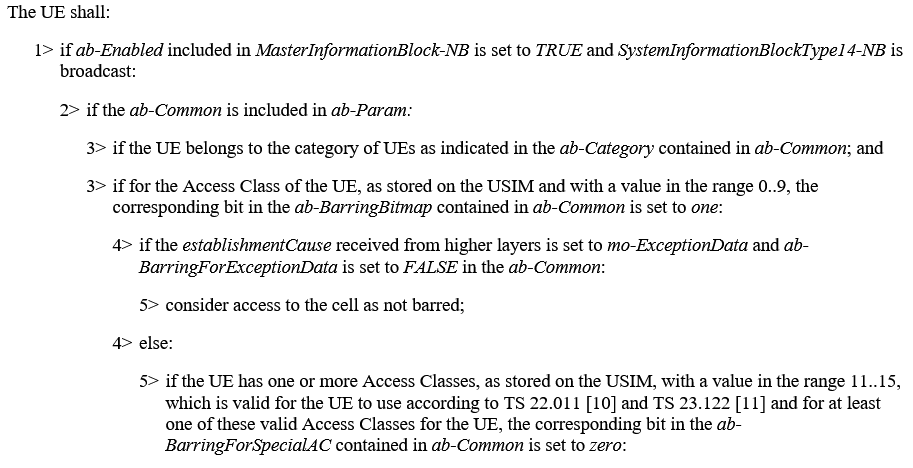
\includegraphics[width=0.7\textwidth]{figures/ab.png}
        \setbeamerfont{caption}{size=\tiny}
    \end{figure}
\end{frame}
\begin{frame}{Background}
\begin{itemize}
    \item {Time is divided in frames, every frame is composed by 10 subframes}
    \item {There are 64 orthogonal preambles in LTE, some of them are reserved for special purposed}
    \begin{itemize}    
        \item[-]{The actual number of available preambles for contention is typically set to 54}
    \end{itemize}
    \item {eNodeB can only detect if a preamble has been actived or not, but not how many device have actually activated it}

\end{itemize}

\end{frame}
%%%%%%%%%%%%%%%%%%%%%%%%%%%%%%%%%%%%%%%%%%%%%%%%%%%%%%
%%%%%%%%%%%%%%%%%%%%%%%%%%%%%%%%%%%%%%%%%%%%%%%%%%%%%%
\section{Proposed solution}
\begin{frame}{{Proposed solution}}
    \begin{itemize}
        \item{Propose to use a q-ary tree splitting algo.}
        \item{It perform through the feedback messages sent by eNodeB}
        \item{propose a new type of MSG4, denoted as MSG4b}
        
    \end{itemize}
\end{frame}
\begin{frame}{{Proposed solution}\\LTE RACH Modification}
    \begin{itemize}
        
        \item{MSG4b specifying the details of the next contention attempt}
        \begin{itemize}    
            \item[-]{MSG4b indicates a set of q preambles to be used for the next contention attemptand the RAO where this contention should take place}
        \end{itemize}
    \end{itemize}
\end{frame}
\begin{frame}{{Proposed solution}\\LTE RACH Modification}
    \begin{figure}[t]
        \centering
        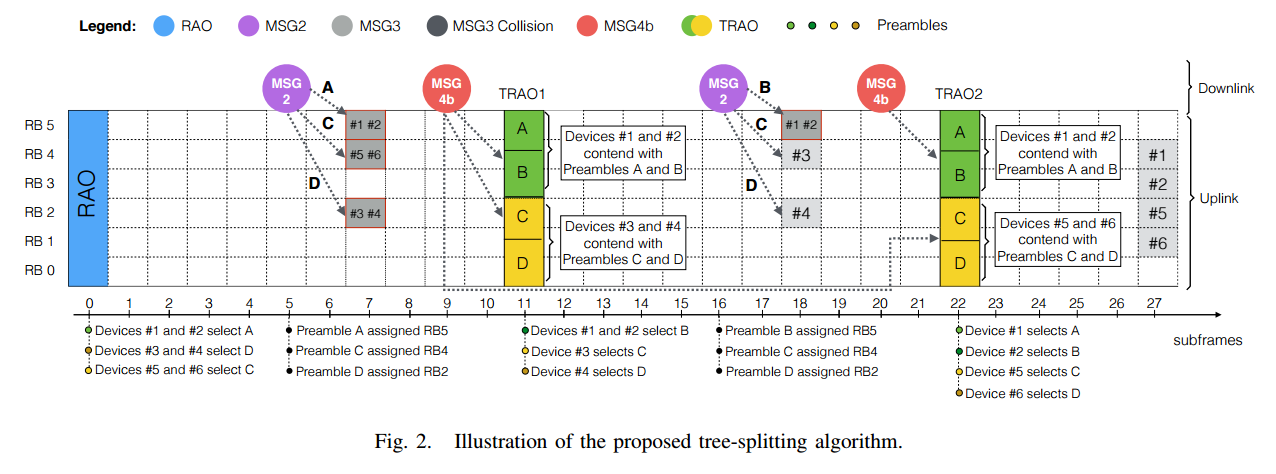
\includegraphics[width=1.1\textwidth]{figures/c.png}
        \setbeamerfont{caption}{size=\tiny}
    \end{figure}
\end{frame}
\begin{frame}{{Proposed solution}\\LTE RACH Modification}
    \begin{figure}[t]
        \centering
        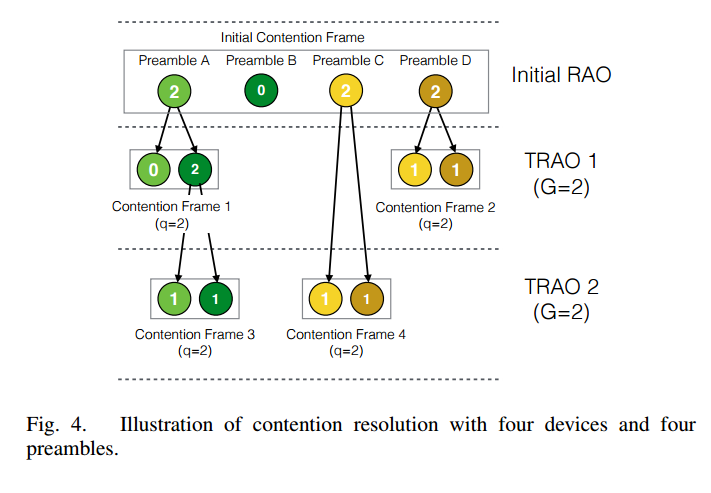
\includegraphics[width=1.1\textwidth]{figures/d.png}
        \setbeamerfont{caption}{size=\tiny}
    \end{figure}
\end{frame}

\section{Result}
\begin{frame}{Result}
    \begin{figure}[t]
        \centering
        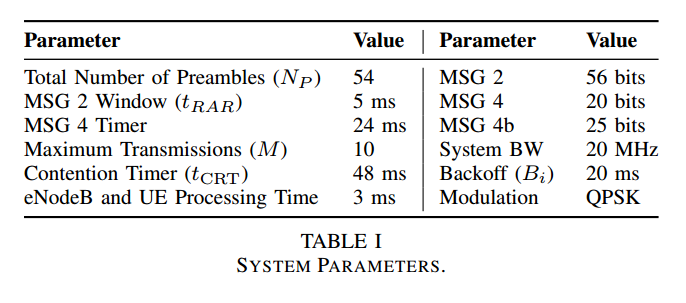
\includegraphics[width=0.8\textwidth]{figures/t.png}
        \setbeamerfont{caption}{size=\tiny}
    \end{figure}
\end{frame}
\begin{frame}{Result}
    \begin{figure}[t]
        \centering
        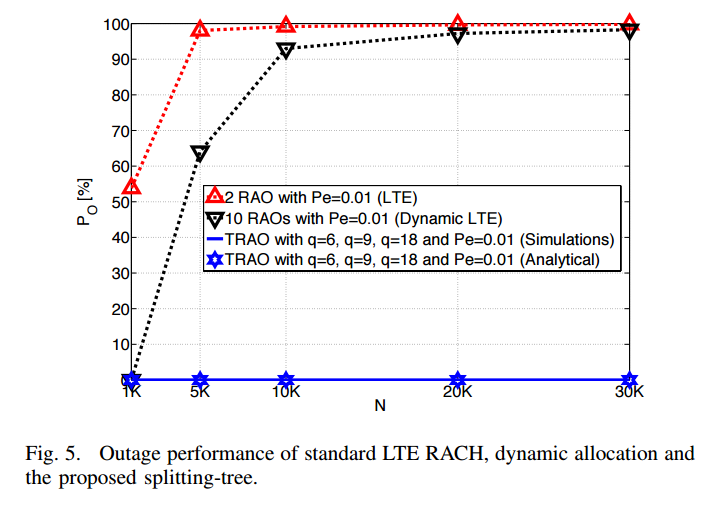
\includegraphics[width=0.8\textwidth]{figures/e.png}
        \setbeamerfont{caption}{size=\tiny}
    \end{figure}
\end{frame}
\begin{frame}{Result}
    \begin{figure}[t]
        \centering
        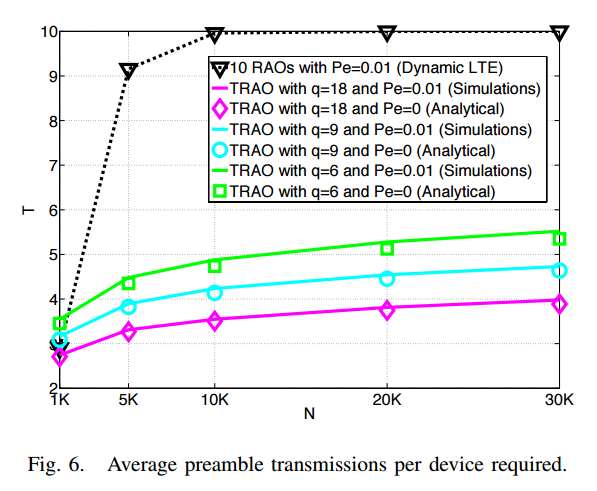
\includegraphics[width=0.8\textwidth]{figures/f.png}
        \setbeamerfont{caption}{size=\tiny}
    \end{figure}
\end{frame}
\begin{frame}{Result}
    \begin{figure}[t]
        \centering
        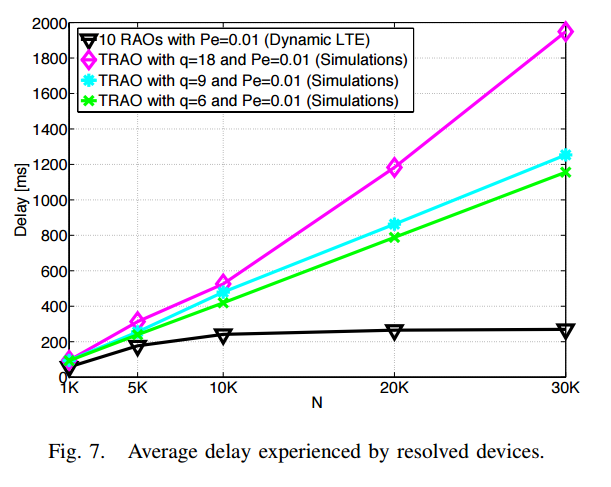
\includegraphics[width=0.8\textwidth]{figures/g.png}
        \setbeamerfont{caption}{size=\tiny}
    \end{figure}
\end{frame}
\begin{frame}{Result}
    \begin{figure}[t]
        \centering
        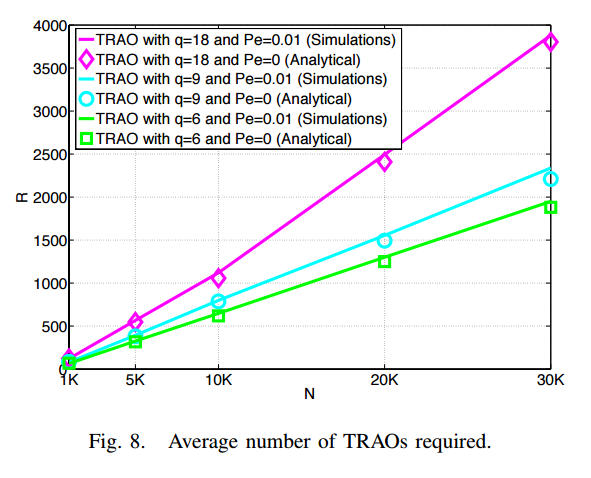
\includegraphics[width=0.8\textwidth]{figures/h.png}
        \setbeamerfont{caption}{size=\tiny}
    \end{figure}
\end{frame}
%%%%%%%%%%%%%%%%%%%%%%%%%%%%%%%%%%%%%%%%%%%%%%%%%%%%%%
%%%%%%%%%%%%%%%%%%%%%%%%%%%%%%%%%%%%%%%%%%%%%%%%%%%%%%
\section{References}
\calcreferencespagetotal % Calc your References Page total number
\begin{frame}[allowframebreaks]{References}
    \fontsize{9pt}{13}\selectfont
    \bibliographystyle{IEEEtran}
    \bibliography{IEEEabrv,Citation}
\end{frame}

%%%%%%%%%%%%%%%%%%%%%%%%%%%%%%%%%%%%%%%%%%%%%%%%%%%%%%
%%%%%%%%%%%%%%%%%%%%%%%%%%%%%%%%%%%%%%%%%%%%%%%%%%%%%%
\section{}

\begin{frame}
    \centering
    \Large{Thanks for Your Attentions}
\end{frame}

\end{document}
